\subsection*{Which Features of \unsafe{} Are Actually Used?}

\begin{figure}[!ht]
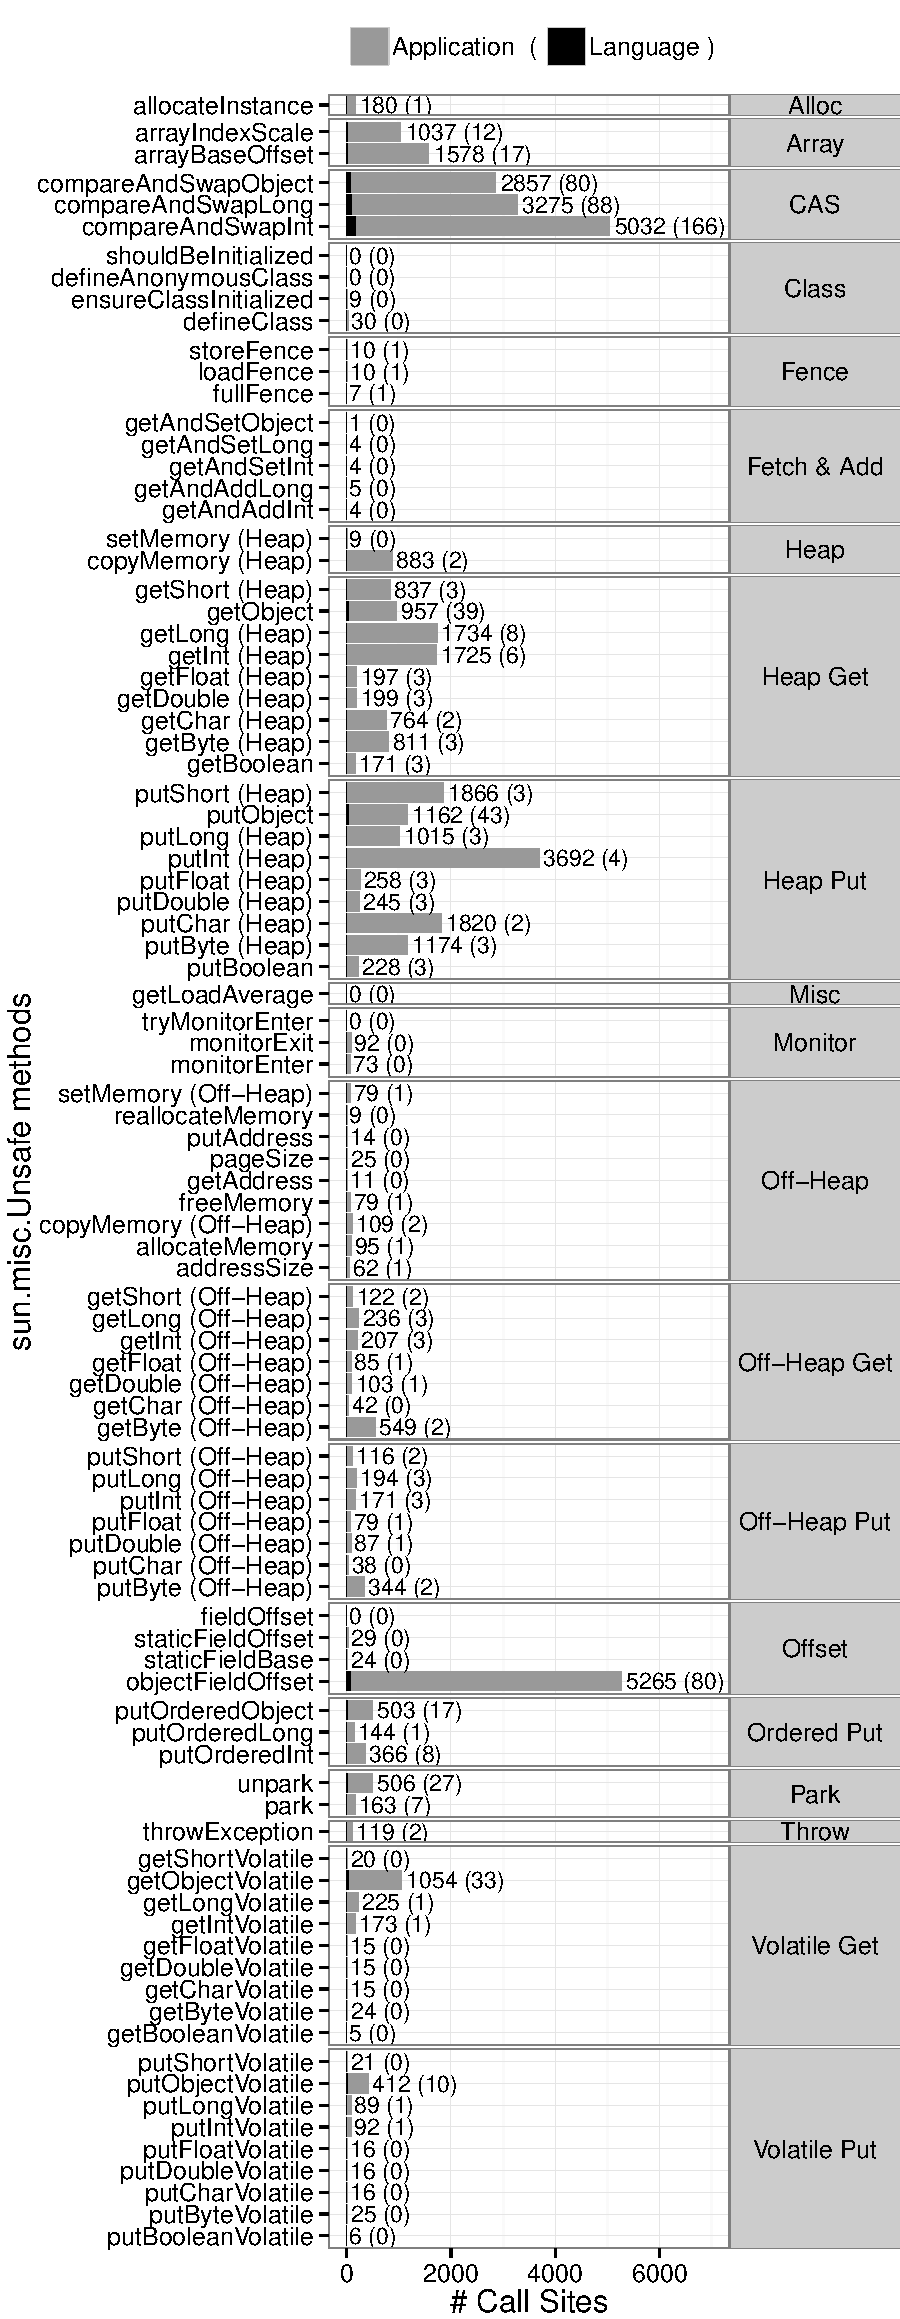
\includegraphics[width=0.5\columnwidth]{chapters/unsafe/usage-maven-methods}
\caption{\smu{} method usage on \mavencentral{}}
\label{fig:overview}
\end{figure}

\begin{figure}[!ht]
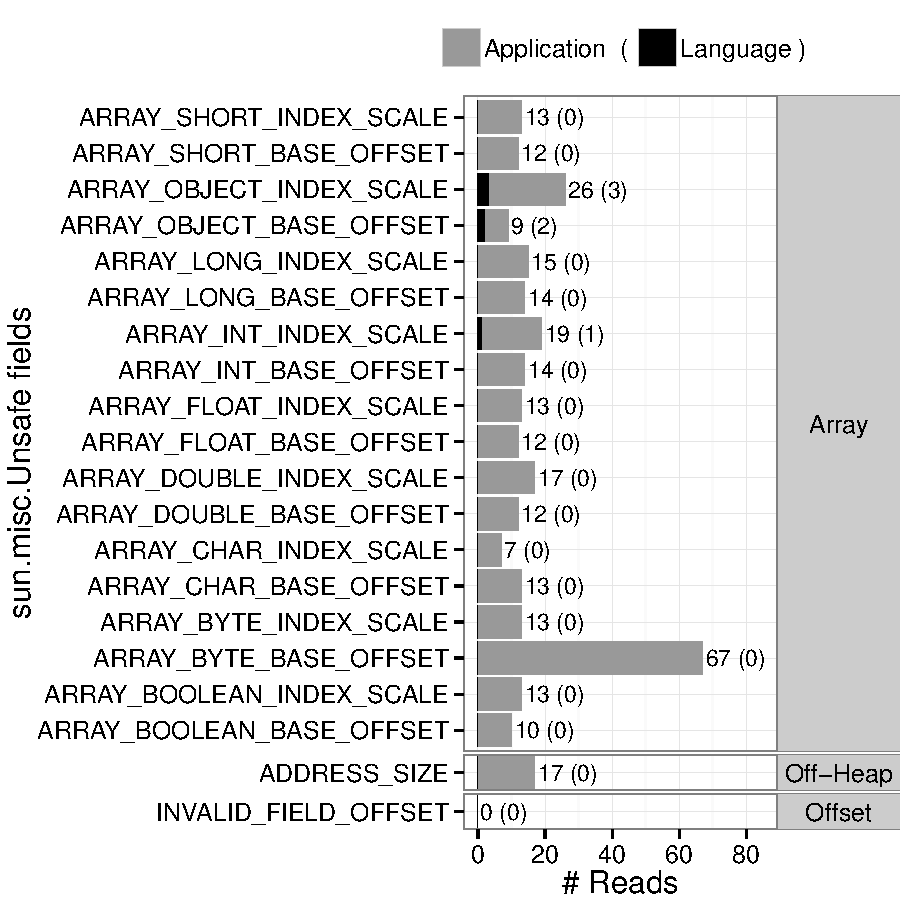
\includegraphics[width=0.7\columnwidth]{chapters/unsafe/usage-maven-fields}
\caption{\smu{} field usage on \mavencentral{}}
\label{fig:overview-field}
\end{figure}

Figures~\ref{fig:overview} and~\ref{fig:overview-field} show all instance methods and static fields of \smu{}. For each member we show how many call sites or field accesses we found across the artifacts. The class provides $120$ public instance methods and $20$ public fields (version 1.8 update 40). The figure only shows $93$ methods because the $18$ methods in the \smugroup{Heap Get} and \smugroup{Heap Put} groups, and \member{staticFieldBase} are overloaded, and we combine overloaded methods into one bar.

We show two columns, \smugroup{Application} and \smugroup{Language}.
The \smugroup{Language} column corresponds to language implementation artifacts while the \smugroup{Application} column corresponds to the rest of the artifacts.

We categorized the members into groups, based on the functionality they provide:

\begin{itemize}
  
\item The \smugroup{Alloc} group contains only the  \member{allocateInstance} method, 
which allows the developer to allocate a \java{} object without executing a constructor.
This method is used 181 times: 180 in \smugroup{Application} and 1 in \smugroup{Language}.

\item The \smugroup{Array} group contains methods and fields for computing relative addresses of array elements.
The fields were added as a simpler and potentially faster alternative in a more recent version of \unsafe{}.
The value of all fields in this group are constants initialized with the result of a call to either \member{arrayBaseOffset} or \member{arrayIndexScale} in the \smugroup{Array} group.
The figures show that the majority of sites still invoke the methods instead of accessing the corresponding constant fields.

\item The \smugroup{CAS} group contains methods to atomically compare-and-swap a \java{} variable. These operations are implemented using processor-specific atomic instructions. For instance, on \emph{x86} architectures, \member{compareAndSwapInt} is implemented using the \texttt{CMPXCHG} machine instruction. Figure~\ref{fig:overview} shows that these methods represent the most heavily used feature of \unsafe{}.

\item Methods of the \smugroup{Class} group are used to dynamically load and check \java{} classes. They are rarely used, with \member{defineClass} being used the most.

\item 
The methods of the \smugroup{Fence} group provide memory fences to ensure loads and stores are visible to other threads.
These methods are implemented using processor-specific instructions.
These methods were introduced only recently in \java{} 8, which explains their limited use in our data set.
We expect that their use will increase over time and that other operations, such as those in the \smugroup{Ordered Put}, or \smugroup{Volatile Put} groups will decrease as programmers use the lower-level fence operations.

\item The \smugroup{Fetch \& Add} group, like the \smugroup{CAS} group, allows the programmer to atomically update a \java{} variable. This group of methods was also added recently in \java{} 8. We expect their use to increase as programmers replace some calls to methods in the \smugroup{CAS} group with the new functionality.

\item The \smugroup{Heap} group methods are used to directly access memory in the \java{} heap. The \smugroup{Heap Get} and \smugroup{Heap Put} groups allow the developer to load and store a Java variable. These groups are among the most frequently used ones in \unsafe{}.

\item The \smugroup{Misc} group contains the method \member{getLoadAverage}, to get the load average in the operating system run queue assigned to the available processors. It is not used.

\item The \smugroup{Monitor} group contains methods to explicitly manage \java{} monitors.
The \member{tryMonitorEnter} method is never used.

\item The \smugroup{Off-Heap} group provides access to unmanaged memory, enabling explicit memory management. Similarly to the \smugroup{Heap Get} and \smugroup{Heap Put} groups, the \smugroup{Off-Heap Get} and \smugroup{Off-Heap Put} groups allow the developer to load and store values in Off-Heap memory. The usage of these methods is non-negligible, with \member{getByte} and \member{putByte} dominating the rest. The value of the \member{ADDRESS\_SIZE} field is the result of the method \member{addressSize()}.

\item Methods of the \smugroup{Offset} group are used to compute the location of fields within \java{} objects. The offsets are used in calls to many other \smu{} methods, for instance those in the \smugroup{Heap Get}, \smugroup{Heap Put}, and the \smugroup{CAS} groups. The method \member{objectFieldOffset} is the most called method in \smu{} due to its result being used by many other \smu{} methods. The \member{fieldOffset} method is deprecated, and indeed, we found no uses.
The \member{INVALID\_FIELD\_OFFSET} field indicates an invalid field offset; it is never used because code using \member{objectFieldOffset} is not written in a defensive style.
%(given that \unsafe{} is used when performance matters, and extra checks might negatively affect performance).


\item 
The \smugroup{Ordered Put} group has methods to store to a \java{} variable without emitting any memory barrier but guaranteeing no reordering across the store.

\item The \member{park} and \member{unpark} methods are contained in the \smugroup{Park} group. With them, it is possible to block and unblock a thread's execution.

\item The \member{throwException} method is contained in the \smugroup{Throw} group, and allows one to throw checked exceptions without declaring them in the \texttt{throws} clause.

\item Finally, the \smugroup{Volatile Get} and \smugroup{Volatile Put} groups allow the developer to store a value in a \java{} variable with \texttt{volatile} semantics.

\end{itemize}

It is interesting to note that despite our large corpus of code, there are several Unsafe methods that are never actually called. If \unsafe{} is to be used in third-party code, then it might make sense to extract those methods into a separate class to be only used from within the runtime library.

%\subsection{Beyond Maven Central}
%
%While Maven Central is a large repository, we wanted to check whether our results generalize to other common repositories. We thus performed a similar analysis of method usage using the \boa{}~\cite{Dyer-Nguyen-Rajan-Nguyen-13} infrastructure. \boa{} allows the developer to mine ASTs of \java{} projects in SourceForge.
%
%The usage profile of Unsafe methods we obtained from \boa{} was similar in shape, but at a different scale, compared to the one obtained from \mavencentral{}. In \boa{}'s SourceForge data, for instance, the most called method, \texttt{objectFieldOffset}, 
%is called 200 times in $50$ projects.
%This is two orders of magnitude lower than the count we found on \mavencentral{}.
%Although \boa{} enables the mining of source code in a convenient way, 
%the SourceForge data it analyzes probably is not current enough 
%to include the more recent Java code that uses \smu{} more heavily.
